\documentclass[../ECON-281-Notes.tex]{subfiles}
\begin{document}
\chapter{Theory of Demand}
In this chapter you will learn
\begin{itemize}
    \item Derivation of the demand curve
    \item price consumption line curve
    \item Income consumption curve
    \item Engle curve
    \item Decomposition of the Price Effect with the substitution and income effect
\end{itemize}

\section{Optimal Choice of Demand}
\subsection{Price Consumption Line}
\begin{Definition}
    {Price Consumption Line}
    Is the set of all utility maximizing points that result from the change in the price of one of the goods while income and the price of the other good are constant.
\end{Definition}


\begin{figure}[htbp]
    \centering
    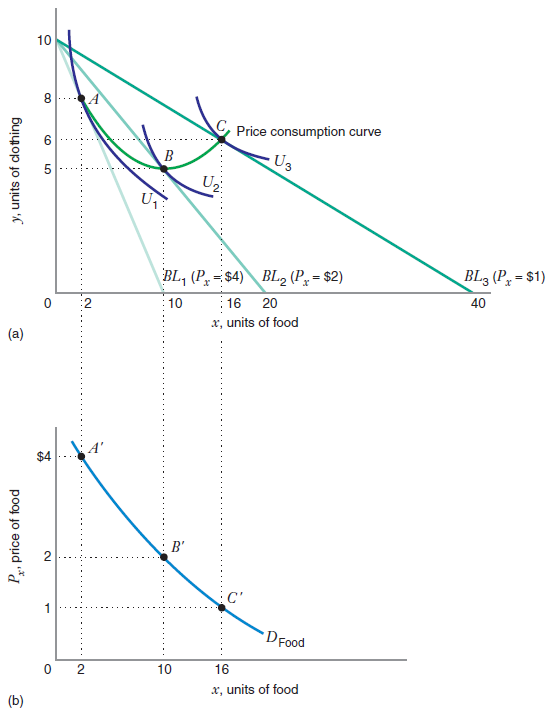
\includegraphics[width=0.8\columnwidth]{../assets/Price-consumption-line.png}
    \caption{Price Consumption Line}
    \label{fig:price-consumption-line}
\end{figure}

As you can see in \cref{fig:price-consumption-line} the price consumption line is positively sloped after a certain point while the demand curve is negatively sloped.

You can also have a vertical price consumption line which could lead to a perfectly inelastic demand curve. This will happen if all the optimal bundles are vertically aligned above each other. 

\subsection{The Effect of a Change in Income}

\begin{Definition}
    {Income Consumption Curve}
    is the set of utility maximizing points that result from the change in income while the prices of teh two goods are kept constant. 
\end{Definition}

\begin{figure}[htbp]
    \centering
    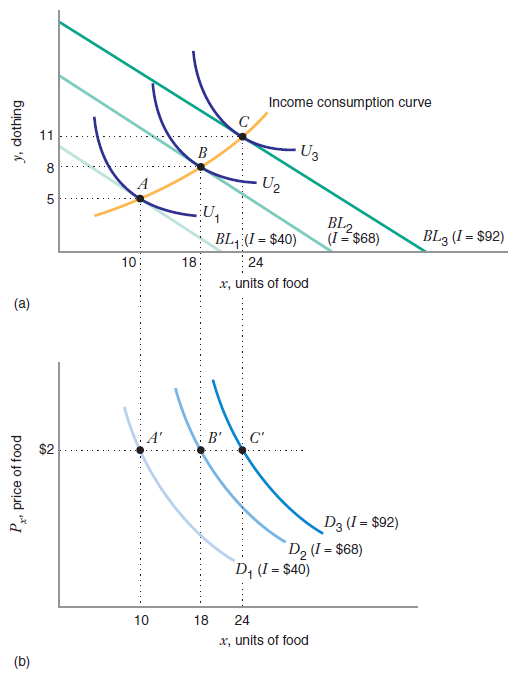
\includegraphics[width=0.8\columnwidth]{../assets/income_consumption_line.png}
    \caption{Income consumption line}
    \label{fig:income_consumption_line}
\end{figure}

A normal good will have a positively sloped income consumption line while an inferior good will have a negatively sloped income consumption line.

\subsubsection{Engel Curve}
\begin{Definition}
    {Engel Curve}
    It shows the relation between quantity demanded and income, while other factors kept constant.
\end{Definition}

A normal good will have a positively sloped Engel curve while an inferior good will have a negatively sloped Engel curve.

\begin{figure}[h!]
    \centering
    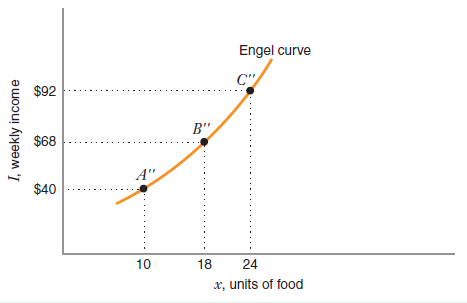
\includegraphics[width=0.8\columnwidth]{../assets/normal_engel_curve.png}
    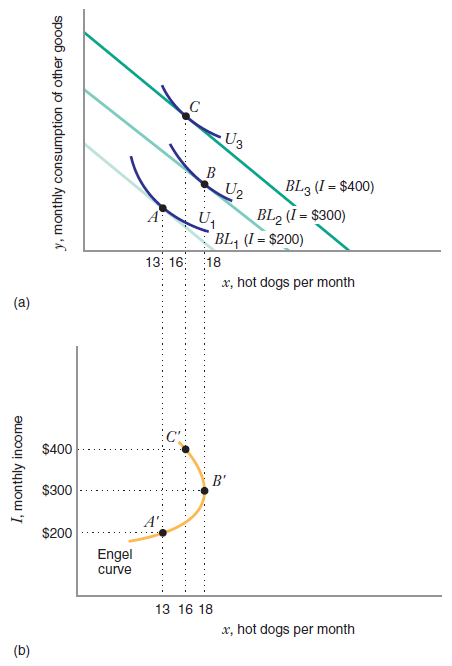
\includegraphics[width=0.8\columnwidth]{../assets/inferior_engel_curve.png}
    \caption{Engel Curve}
    \label{fig:engel_curve}
\end{figure}
\newpage

\section{Effect of a Change in the Price}
When there is a change in the price there is a negative correlation with quantity demanded. This effect is called the \textbf{Price Effect} and is comprised with two other effects. 
\begin{itemize}
    \item \textbf{Substitution Effect}: What is the substitution of the good when your real purchasing power is kept the same but the price of good changes. 
    \item \textbf{Income Effect}: What is the purchasing effect of the good when your real purchasing power increases. i.e., is the good normal or inferior.
\end{itemize}

\subsubsection{Steps to calculate Price Effect}

\begin{figure}[t]
    \centering
    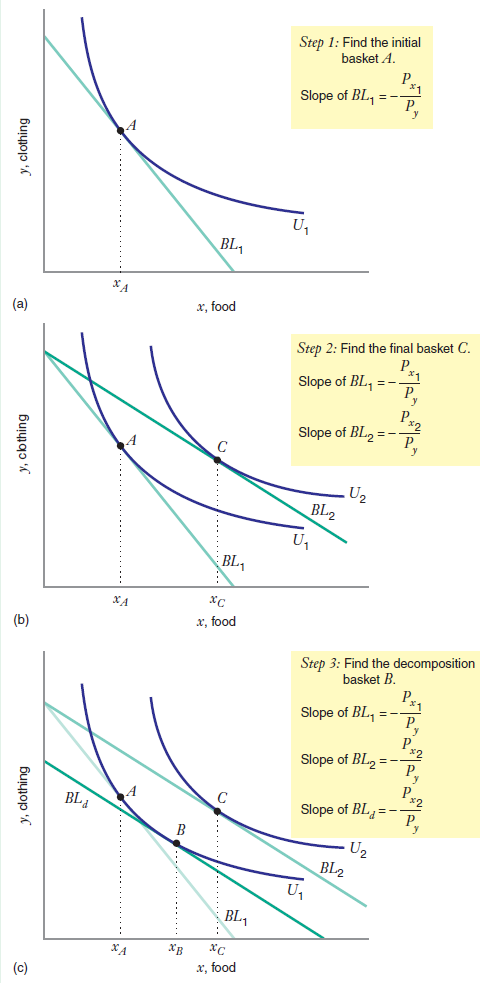
\includegraphics[width=0.8\columnwidth]{../assets/PE-steps.png}
    \caption{Steps to Calculate Price Effect}
    \label{fig:calc_price_effect}
\end{figure}

In \cref{fig:calc_price_effect} subgraph a you have the initial bundle at the original price. Then either the price of good x increases or decreases, in the figure it decrease rotating the new budget line outwards in subgraph b. This will give you the Price Effect of good, to decompose it into it's constitute parts, you make an imaginary budget line that is parallel to the new budget line but it's tangent to the original indifference curve as shown in subgraph c. Point B is the point of tangency that separates the Income Effect and the Substitution Effect. The distance from Point A and B is caused by the substitution effect as your real purchasing power is kept the same, while the distance from point B to C is caused by the Income Effect, the effect caused by the increase in purchasing power. 


\begin{figure}[t]
    \centering
    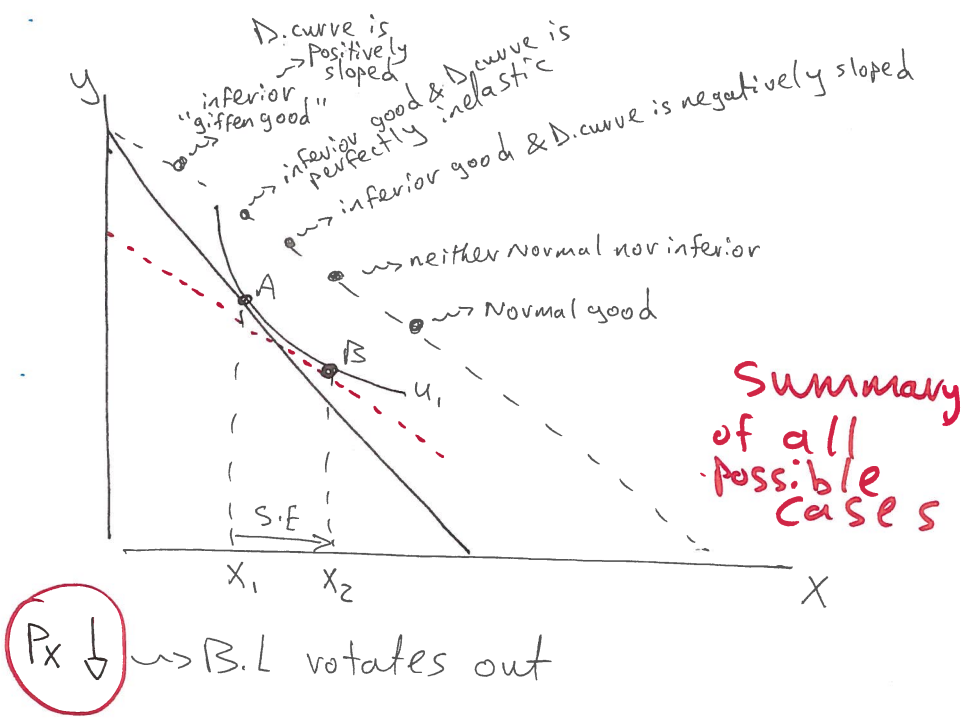
\includegraphics[width=\columnwidth]{../assets/PE-decrease-all.png}
    \\~\\
    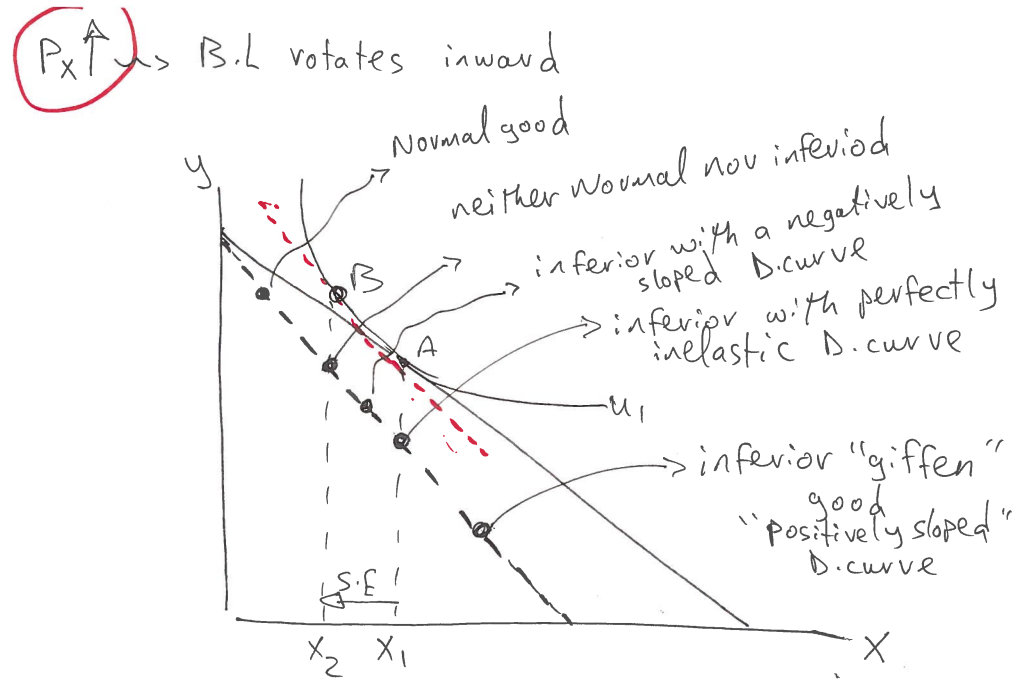
\includegraphics[width=\columnwidth]{../assets/PE-increase-all.png}
    \caption{All Price Effect Cases in one}
    \label{fig:all_pe_in_one}
\end{figure}

\Cref{fig:all_pe_in_one} shows the five cases where the new optimal bundle can be located after a change in price. 

\begin{Definition}
    {Giffen Good}
    A \textbf{Giffen Good} is a type of inferior good where the demand curve is positively sloped. That is the higher the price, the higher the quantity demanded.
\end{Definition}

\section{Market Demand with Network Externalities}
Your demand or consumption is affected by other consumers who buys the same good. 
There are two effects we will look at
\begin{itemize}
    \item \textbf{Bandwagon Effect}: Your demand increases when more people buys the good
    \item \textbf{Snob Effect}: Your demand decreases when more people buys the good
\end{itemize}
\begin{figure}[!t]
    \centering
    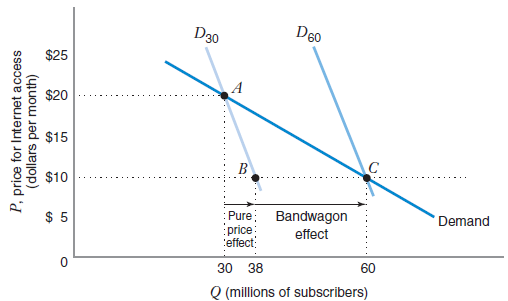
\includegraphics[width=\columnwidth]{../assets/bandwagon.png}
    \caption{Bandwagon Effect}
    \label{fig:bandwagon_effect}
\end{figure}

\begin{figure}[!t]
    \centering
    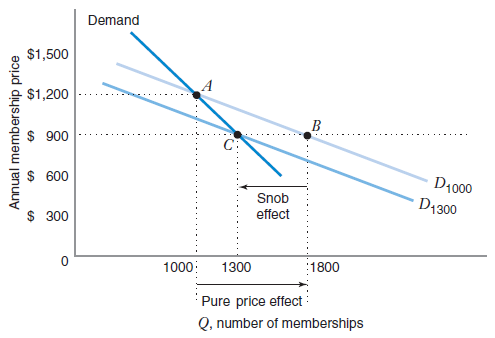
\includegraphics[width=\columnwidth]{../assets/snob.png}
    \caption{Snob Effect}
    \label{fig:snob_effect}
\end{figure}


\end{document}